\Aeqref{airy:airyeq} egyenlet \eqref{3dbox:1deq} alakúra hozható a
\begin{equation}
	x = ax^\prime - bE,
\end{equation}
\begin{equation}
	y(x) = y(ax^\prime - bE)
\end{equation}
helyettesítésekkel. A helyettesítés után $\frac{d}{dx} = \frac{1}{a}\frac{d}{dx^\prime}$, és \aeqref{airy:airyeq} alakja
\begin{equation}
	\frac{d^2y(ax-bE)}{{dx^\prime}^2} - \left(a^3x - a^2bE\right)y(ax-bE) = 0.
\end{equation}
Ezt az egyenletet összevetve \eqref{3dbox:1deq} egyenlettel $a$ és $b$ értéke leolvasható,
\begin{equation}
	a = \sqrt[3]{\frac{2mF}{\hbar^2}},
\end{equation}
\begin{equation}
	b = \sqrt[3]{\frac{2m}{\hbar^2F^2}}.
\end{equation}
Az egy dimenziós időfüggetlen Schrödinger egyenlet megoldása
\begin{equation}
	\psi(x) = c_1\Ai(ax-bE)+c_2\Bi(ax-bE),
\end{equation}
melyet a határfeltételekhez kell illeszteni,
\begin{equation}
	\psi(0) = \psi(L) = 0.
\end{equation}
A $\psi(0) = 0$ feltételből következik, hogy $\psi \propto \Bi(-bE)\Ai(ax-bE) - \Ai(-bE)\Bi(ax-bE)$. A második határfeltétel pedig meghatározza a lehetséges energiákat,
\begin{equation}
		0 = \psi(L) = \Bi(-bE)\Ai(aL-bE) - \Ai(-bE)\Bi(aL-bE).
\end{equation}
Felhasználva a $\Ti(x)$ függvényt, az egyenlet kompakt és jól közelíthető alakra hozható,
\begin{equation}
	\label{box_energiaszintek_egyenlet}
	\Ti(aL-bE) - \Ti(-bE) = 0.
\end{equation}
\begin{figure}[H]
	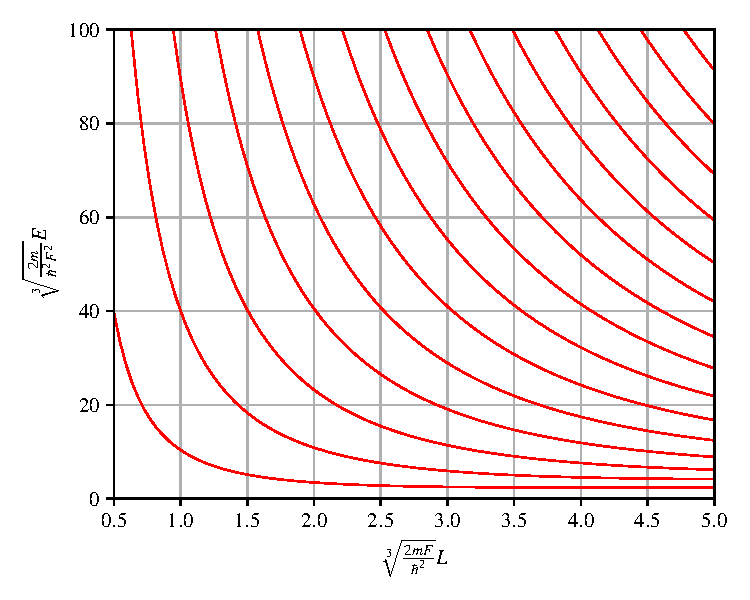
\includegraphics[scale=1]{./figs/energiaszintek.pdf}
	\caption[Egzakt energiaszintek]{Egzakt energia szintek, $bE$ és $aL$ közötti relációval ábrázolva. Az ába jobb alsó sarkán látható, hogy $E \ll FL$ esetén az energiaszintek $L$-től függetlenek lesznek, mivel a félvégtelen tér beli homogén tér energiaszintjeit közelítik.}
	\label{box_energiaszintek_abra}
\end{figure}
Amikor $FL \ll \frac{\pi^2\hbar^2}{2mL^2}$, a potenciál jól közelíthető konstans potenciállal, mivel az alapállapot energiájához képest is elhanyagolható a lineáris potenciál eltérése a konstans potenciáltól. Eben a esetben $E \propto n^2$. $E \ll FL$ esetben az energiaszintek jó közelítéssel konstanssá válnak. Ennek az oka, hogy $\lim_{L \to \infty}\psi(x) = \alpha \Ai\left(ax-b\right)$, mert a $\Bi\left(x\right)$ exponenciálisan növekszik nagy $x$-ek esetén. Ebben az eseten az energiaszinteket a $\Ai(-bE) = 0$ egyenlet határozza meg. Ezeket az aszimptotikus viselkedéseket \aref{box_energiaszintek_abra}. ábra jól mutatja, később a Szemiklasszikus közelítés tárgyalása közben az aszimptotikus .
	
	
%A probléma egy 1D dobozba zárt résecske homogén erőtérben. $F(x)=-F$, azaz $V(x) = Fx$.
%	Az egyenlethez tartozó határfeltételek, ha a doboz hossza $L$:
%	\begin{equation}
%		\phi \big\rvert_0 = \phi \big \rvert_L = 0
%	\end{equation}
%	A megoldandó időfüggetlen Schrödinger-egyenlet:
%	\begin{equation}
%		-\frac{\hbar^2}{2m}\frac{d^2\phi}{dx^2} + Fx\phi = E\phi
%	\end{equation}
%	\begin{equation}
%		\frac{d^2\phi}{dx^2} - \frac{2mFx}{\hbar^2}\phi = -\frac{2mE}{\hbar^2}\phi
%	\end{equation}
%	\begin{equation}
%		\frac{d^2\phi}{dx^2} - \left(\frac{2mF}{\hbar^2}x - \frac{2mE}{\hbar^2}\right)\phi = 0
%	\end{equation}
%	Az Airy egyenlet ilyen alakra hozható a változó affin lineáris transzformációjával:
%	\begin{equation}
%		\frac{d^2y}{dx^{\prime 2}} - x^\prime y = 0
%	\end{equation}
%	$x^\prime = ax - bE$, azaz $\frac{d}{dx} = a\frac{d}{dx^\prime}$:
%	\begin{equation}
%		\frac{d^2y}{dx^2} - \left(a^3x - a^2bE\right)y = 0
%	\end{equation}
%	Az együtthatók összevetése alapján $a = \sqrt[3]{\frac{2mF}{\hbar^2}}$ és $b = \sqrt[3]{\frac{2m}{\hbar^2F^2}}$. Így a Schrödinger-egyenlet megoldása:
%	\begin{equation}
%		\phi(x) = y(x^\prime) = y\left(\sqrt[3]{\frac{2mF}{\hbar^2}}x - \sqrt[3]{\frac{2m}{\hbar^2F^2}}E\right)
%	\end{equation}
%	, ahol $y(x) = \alpha \Ai\left(x\right) + \beta \Bi\left(x\right)$.
%	A $\phi \big\rvert_0 = 0$ feltételből következik, hogy $\phi \propto \Bi\left(-bE\right)\Ai\left(ax-bE\right) - \Ai\left(-bE\right)\Bi\left(ax-bE\right)$. A második határfeltétel pedig meghatározza a lehetséges energiákat. A feltétel:
%	\begin{equation}
%		\Bi\left(-bE\right)\Ai\left(aL-bE\right) - \Ai\left(-bE\right)\Bi\left(aL-bE\right) = 0
%	\end{equation}
%	\begin{equation}
%		\label{box_energiaszintek_egyenlet}
%		\Ti{aL-bE} - \Ti{-bE} = 0
%	\end{equation}
%	\begin{equation}
%		\Ti{\sqrt[3]{\frac{2mF}{\hbar^2}}L - \sqrt[3]{\frac{2m}{\hbar^2F^2}}E} - \Ti{-\sqrt[3]{\frac{2m}{\hbar^2F^2}}E} = 0
%	\end{equation}
%	\begin{figure}[H]
%		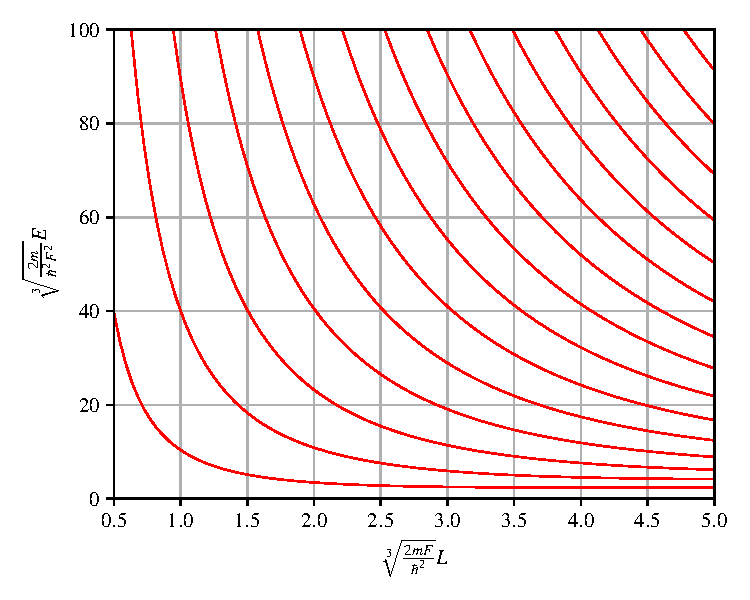
\includegraphics[scale=1]{./figs/energiaszintek.pdf}
%		\caption[Egzakt energiaszintek]{Egzakt energia szintek, $bE$ és $aL$ közötti relációval ábrázolva. Az ába jobb alsó sarkán látható, hogy $E \ll FL$ esetén az energiaszintek $L$-től függetlenek lesznek, mivel a félvégtelen tér beli homogén tér energiaszintjeit közelítik.}
%		\label{box_energiaszintek_abra}
%	\end{figure}
%	Amikor $FL \ll \frac{\pi^2\hbar^2}{2mL^2}$, a potenciál jól közelíthető konstans potenciállal, mivel az alapállapot energiájához képest is elhanyagolható a lineáris potenciál eltérése a konstans potenciáltól. Eben a esetben $E \propto n^2$. $E \ll FL$ esetben az energiaszintek jó közelítéssel konstanssá válnak. Ennek az oka, hogy $\lim_{L \to \infty}\psi(x) = \alpha \Ai\left(ax-b\right)$, mert a $\Bi\left(x\right)$ exponenciálisan növekszik nagy $x$-ek esetén. Ebben az eseten az energiaszinteket a $\Ai\left(- \sqrt[3]{\frac{2m}{\hbar^2F^2}}E\right) = 0$ egyenlet határozza meg. Ezeket az aszimptotikus viselkedéseket \aref{box_energiaszintek_abra}. ábra jól mutatja.
%    
%    TODO: link 1D videóról
%